\documentclass[hyperref, a4paper]{article}

\usepackage{geometry}
\usepackage{titling}
\usepackage{titlesec}
% No longer needed, since we will use enumitem package
% \usepackage{paralist}
\usepackage{enumitem}
\usepackage{footnote}
\usepackage[colorinlistoftodos]{todonotes}
\usepackage{amsmath, amssymb, amsthm}
\usepackage{mathtools}
\usepackage{bbm}
\usepackage{graphicx}
\usepackage{subcaption}
\usepackage{soulutf8}
\usepackage{physics}
\usepackage{tensor}
\usepackage{siunitx}
\usepackage[version=4]{mhchem}
\usepackage{tikz}
\usepackage{xcolor}
\usepackage{listings}
\usepackage{autobreak}
\usepackage[ruled, vlined, linesnumbered]{algorithm2e}
\usepackage{nameref,zref-xr}
\zxrsetup{toltxlabel}
\usepackage[backend=bibtex,sorting=none]{biblatex}
\addbibresource{arpes.bib}
\usepackage[colorlinks,unicode]{hyperref} % , linkcolor=black, anchorcolor=black, citecolor=black, urlcolor=black, filecolor=black
\usepackage[most]{tcolorbox}
\usepackage{prettyref}

% Page style
\geometry{left=3.18cm,right=3.18cm,top=2.54cm,bottom=2.54cm}
\titlespacing{\paragraph}{0pt}{1pt}{10pt}[20pt]
\setlength{\droptitle}{-5em}

% More compact lists 
\setlist[itemize]{
    itemindent=17pt, 
    leftmargin=1pt,
    listparindent=\parindent,
    parsep=0pt,
}

% Math operators
\DeclareMathOperator{\timeorder}{\mathcal{T}}
\DeclareMathOperator{\diag}{diag}
\DeclareMathOperator{\legpoly}{P}
\DeclareMathOperator{\primevalue}{P}
\DeclareMathOperator{\sgn}{sgn}
\DeclareMathOperator{\res}{Res}
\newcommand*{\ii}{\mathrm{i}}
\newcommand*{\ee}{\mathrm{e}}
\newcommand*{\const}{\mathrm{const}}
\newcommand*{\suchthat}{\quad \text{s.t.} \quad}
\newcommand*{\argmin}{\arg\min}
\newcommand*{\argmax}{\arg\max}
\newcommand*{\normalorder}[1]{: #1 :}
\newcommand*{\pair}[1]{\langle #1 \rangle}
\newcommand*{\fd}[1]{\mathcal{D} #1}
\DeclareMathOperator{\bigO}{\mathcal{O}}

% TikZ setting
\usetikzlibrary{arrows,shapes,positioning}
\usetikzlibrary{arrows.meta}
\usetikzlibrary{decorations.markings}
\tikzstyle arrowstyle=[scale=1]
\tikzstyle directed=[postaction={decorate,decoration={markings,
    mark=at position .5 with {\arrow[arrowstyle]{stealth}}}}]
\tikzstyle ray=[directed, thick]
\tikzstyle dot=[anchor=base,fill,circle,inner sep=1pt]

% Algorithm setting
% Julia-style code
\SetKwIF{If}{ElseIf}{Else}{if}{}{elseif}{else}{end}
\SetKwFor{For}{for}{}{end}
\SetKwFor{While}{while}{}{end}
\SetKwProg{Function}{function}{}{end}
\SetArgSty{textnormal}

\newcommand*{\concept}[1]{{\textbf{#1}}}

% Embedded codes
\lstset{basicstyle=\ttfamily,
  showstringspaces=false,
  commentstyle=\color{gray},
  keywordstyle=\color{blue}
}

% Reference formatting
\newcommand*{\citesec}[1]{\S~{#1}}
\newcommand*{\citechap}[1]{chap.~{#1}}
\newcommand*{\citefig}[1]{Fig.~{#1}}
\newcommand*{\citetable}[1]{Table~{#1}}
\newcommand*{\citepage}[1]{pp.~{#1}}
\newrefformat{fig}{Fig.~\ref{#1}}
\newcommand*{\term}[1]{\textit{#1}}

% Color boxes
\tcbuselibrary{skins, breakable, theorems}

\newtcbtheorem{infobox}{Box}{
    enhanced,
    boxrule=0pt,
    colback=blue!5,
    colframe=blue!5,
    coltitle=blue!50,
    borderline west={4pt}{0pt}{blue!65},
    sharp corners,
    fonttitle=\bfseries, 
    breakable,
    before upper={\parindent15pt\noindent}}{box}
\newtcbtheorem[use counter from=infobox]{theorybox}{Box}{
    enhanced,
    boxrule=0pt,
    colback=orange!5, 
    colframe=orange!5, 
    coltitle=orange!50,
    borderline west={4pt}{0pt}{orange!65},
    sharp corners,
    fonttitle=\bfseries, 
    breakable,
    before upper={\parindent15pt\noindent}}{box}
\newtcbtheorem[use counter from=infobox]{learnbox}{Box}{
    enhanced,
    boxrule=0pt,
    colback=green!5,
    colframe=green!5,
    coltitle=green!50,
    borderline west={4pt}{0pt}{green!65},
    sharp corners,
    fonttitle=\bfseries, 
    breakable,
    before upper={\parindent15pt\noindent}}{box}


\newenvironment{shelldisplay}{\begin{lstlisting}}{\end{lstlisting}}

\newcommand*{\kB}{k_{\text{B}}}
\newcommand*{\muB}{\mu_{\text{B}}}
\newcommand*{\efermi}{E_{\text{F}}}
\newcommand*{\pfermi}{p_{\text{F}}}
\newcommand*{\vfermi}{v_{\text{F}}}
\newcommand*{\sA}{\text{A}}
\newcommand*{\sB}{\text{B}}
\newcommand*{\Tc}{T_{\text{c}}}
\newcommand*{\hethree}{$^3$He}
\newcommand*{\hefour}{$^4$He}
\newcommand{\epsr}{\epsilon_{\text{r}}}
\newcommand{\chie}{\chi_{\text{e}}}
\newcommand{\Efreq}{\tilde{\vb*{E}}}
\newcommand{\Dfreq}{\tilde{\vb*{D}}}
\newcommand{\Pfreq}{\tilde{\vb*{P}}}

\title{Preliminary results on trion signature in time-resolved ARPES}
\author{}
\date{}

\begin{document}

\maketitle

When the temporal separation between the pump and the probe is long enough,
the effect of the pump is essentially preparing an initial state 
with various excitations, 
which are then detected by the probe.
The probe drives the electron part(s) of an excitation out the material, 
which then contributes to the total ARPES intensity;
since the electrons in the excitations always reside on conduction bands, 
they leave signatures in the resulting ARPES spectrum 
that are absent in conventional ARPES.
The probability to detect an electron with momentum $\vb{k}$ 
from an excitation $\ket*{\Psi_n}$ at time $t$
is given as \cite{rustagi2018photoemission}
\begin{equation}
    P_{\vb{k}}(\omega, t) = \sum_{c, \vb{k}'}
    { \abs*{M^{fc}_{\vb{k} \vb{k}'}}^2 }
    \int_{t_0}^t \dd{t_1} \int_{t_0}^t \dd{t_2}
    { \ee^{-\ii (E_n - \omega ) (t_1 - t_2)}} 
    { \mel{\Psi_n(t_0)}{c^\dagger_{\vb{k}'} 
    U(t_2, t_1) c_{\vb{k}'}}{\Psi_n(t_0)}}
    { s(t_1) s(t_2)},
    \label{eq:arpes-pure-state}
\end{equation}
where $t_0$ is the time the probe starts,
$\omega$ is the energy of the out-coming electron 
plus the work function minus the photon energy, 
$E_n$ is the energy of $\ket*{\Psi_n(t)}$,
$c$ is a band index in the material, 
$c_{\vb{k}'}$ refers to the annihilation operator of that mode, 
$M_{\vb{k} \vb{k}'}^{fc}$ is the dipole transition matrix 
between the $(c, \vb{k}')$ band electron state in the material and 
the outgoing final state $(f, \vb{k})$,
$U(t_2, t_1)$ is the many-body time evolution operator in the material,
and $s(t)$ is the shape of the probe pulse.
The time evolution operator carries information regarding 
the oscillation of the state of the system after one electron is kicked out,
leading to a broadened form of energy conservation 
after the integrations over $t_1$ and $t_2$ are finished
that determines the shape of the ARPES signature.
It is possible that the final state of pumping is a mixed state 
of several excitations, 
and in this case \eqref{eq:arpes-pure-state} needs to be 
averaged over the probabilistic distribution of the excitations,
and the excitation signatures are overlaid to each other.

In the case of two-dimensional materials, $\vb{k}_\parallel = \vb{k}'$.
Within the framework of the two-band model, 
it has been shown~\cite{rustagi2018photoemission} that 
the signature of an exciton has the dispersion relation of
\begin{equation}
    \omega = E_{S \vb{Q}} + \epsilon_{v \vb{k}_\parallel - \vb{Q}},
\end{equation}
where $E_{S \vb{Q}}$ is the single exciton energy, 
i.e. band gap plus the negative binding energy.
In the case of a positive trion, 
there is no single, definite dispersion relation that determines the shape of the ARPES signature;
assuming that after one electron is driven out, 
scatterings between the two remaining holes are negligible, 
the dispersion of the trion ARPES signature is determined by the following family of curves 
\begin{equation}
    \omega = E_{S \vb{P}} + \epsilon_{v \vb{k}_{\text{h1}}} + \epsilon_{v \vb{k}_{\text{h2}}}, \quad 
    \vb{k}_\parallel - \vb{k}_{\text{h1}} - \vb{k}_{\text{h2}} = \vb{P}.
\end{equation}
In \prettyref{fig:arpes-exciton-trion}, it could be observed that 
in the zero-temperature case,
even when a trion mode and an exciton mode with the same energy,
they still result in different ARPES signatures:
the slopes and curvatures of the ARPES signature are different, 
and when the total momentum of the excitation is given, 
the position shifts of the signature on the ARPES heatmap are also different.

\begin{figure}
    \centering
    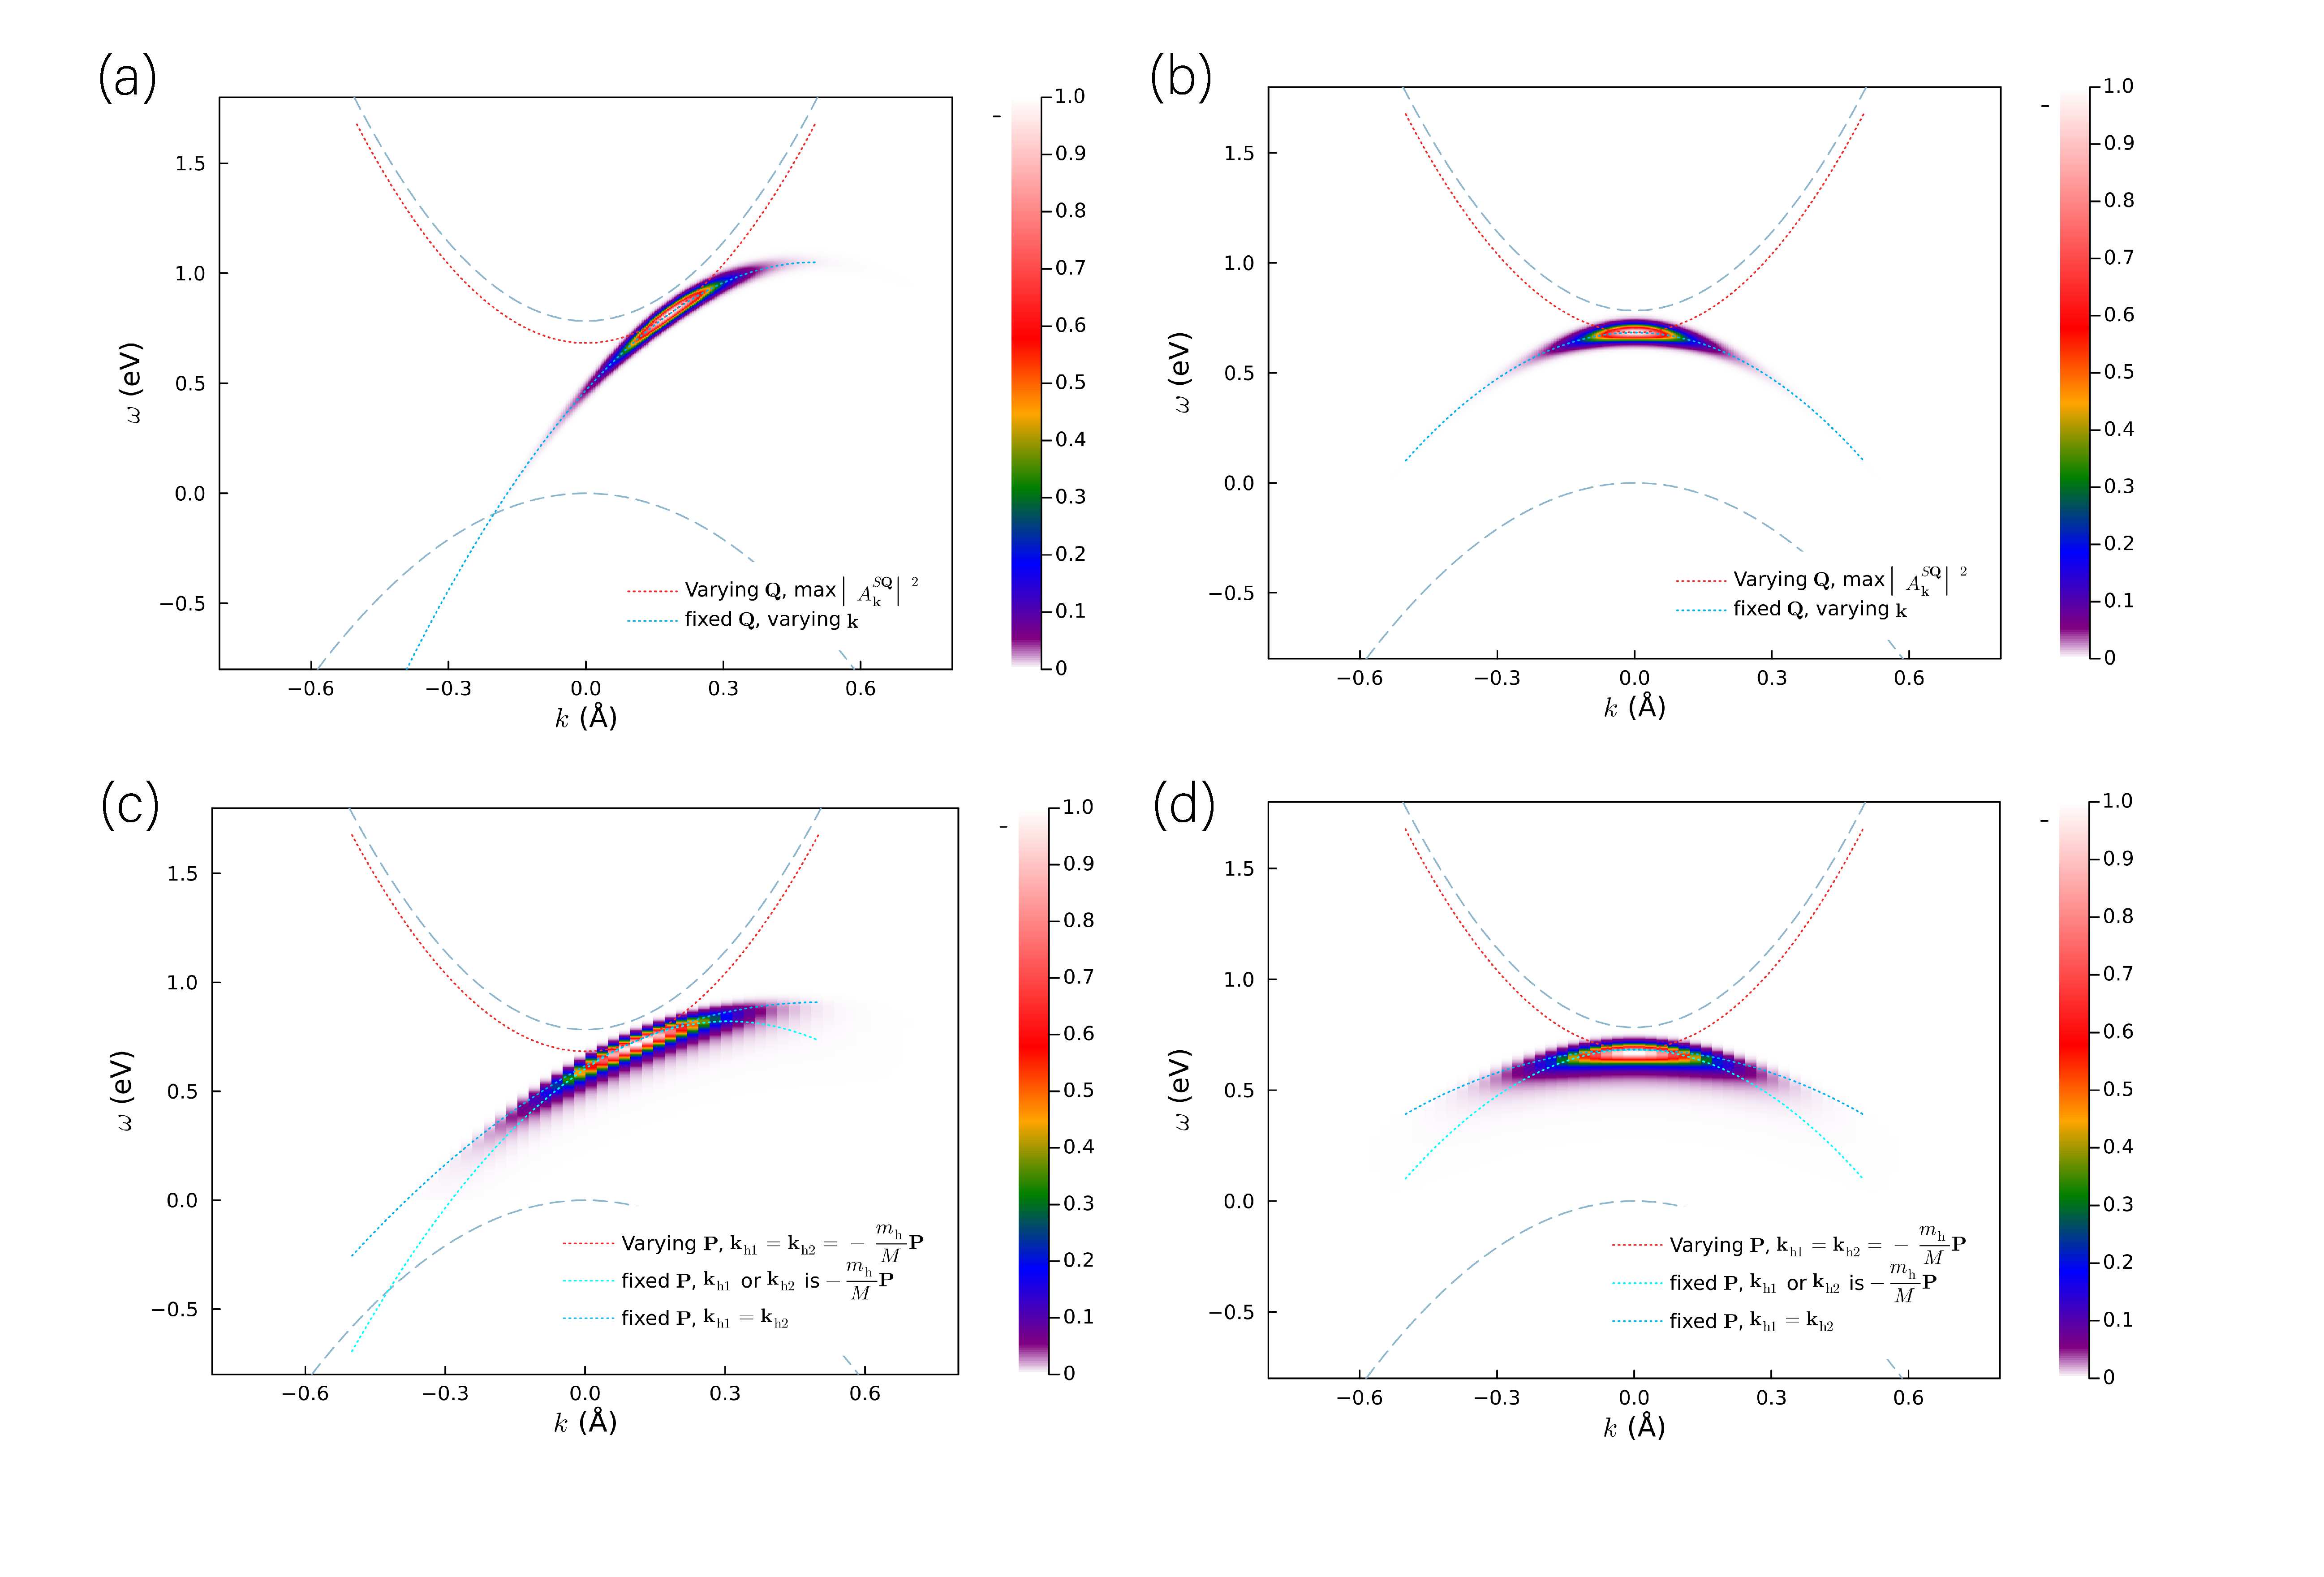
\includegraphics[width=0.9\textwidth]{images/exciton-trion-comparison.pdf}
    \caption{Comparison between exciton signatures and trion signatures.}
    \label{fig:arpes-exciton-trion}
\end{figure}

\printbibliography

\end{document}